\section{Implementation med event sourcing}
Event sourcing er implementeret for bedre at adskille read og write modellen. Samt opnå eventual consistency.
Domæne delen er fjernet. Dvs. der ikke længere er gemt nogen entities. Tilgængel gemmes alle commands.
For at lave en entity må en read model selv skabe den, ved at kombinere alle relevante commands.
I dette projekt er defineret fire commands: AddUser, RenameUser, AddGroup og JoinGroup.
\begin{figure}[H]
	\center
	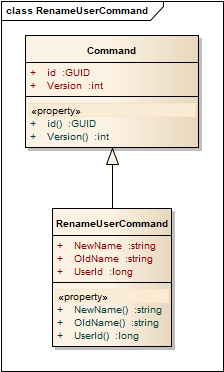
\includegraphics[width=0.25\textwidth]{RenameUserCommand.png}
	\caption{Eksempel på RenameUserCommand}
	\label{fig:RenameUserCommandl}
\end{figure}
Dette betyder at f.eks. en read model som gerne vil have alle brugere, med navn. Bliver nød til at kombinere én AddUser command med alle tilhørende RenameUser commands.
En read model som er interesseret i grupper. Kunne nøjes med at kigge på AddGroup. Men hvis read modellen også er interesseret i gruppens medlemmer. Skal alle tilhørende JoinGroup commands gennemgås.
\newline
I write modellen indsættes RenameUser command via en handler.
\lstinputlisting[language=C]{Kode/RenameUserHandler.cs}


